\documentclass{standalone}
\usepackage{tikz}

\begin{document}

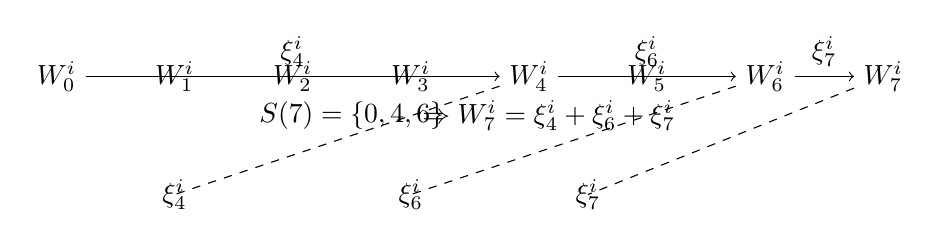
\begin{tikzpicture}[node distance=2cm]
    % Nodes
    \foreach \i in {0,...,7}{
        \node (W\i) at (\i*1.5,0) {$W_\i^i$};
    }
    
    % Edges
    \draw[->] (W0) -- node[above]{$\xi_4^i$} (W4);
    \draw[->] (W4) -- node[above]{$\xi_6^i$} (W6);
    \draw[->] (W6) -- node[above]{$\xi_7^i$} (W7);
    
    % Path labels
    \node at (3.75,-0.5) {$\mc S(7) = \{0, 4, 6\}$};
    \node at (6.25,-0.5) {$\Rightarrow W_7^i = \xi_4^i + \xi_6^i + \xi_7^i$};
    
    % Gaussian nodes
    \node at (1.5,-1.5) {$\xi_4^i$};
    \node at (4.5,-1.5) {$\xi_6^i$};
    \node at (6.75,-1.5) {$\xi_7^i$};
    
    % Lines connecting Gaussian nodes to their respective \( W \)
    \draw[dashed] (W4) -- (1.5,-1.5);
    \draw[dashed] (W6) -- (4.5,-1.5);
    \draw[dashed] (W7) -- (6.75,-1.5);
\end{tikzpicture}

\end{document}